\section{接触阶段与分离边界}
\subsection{支持力为零之前必须使用接触方程}
两个物体接触时，法向几何关系限制它们的相对加速度，支持力负责实现这个限制。分离不是事先另指定的一种运动，而是接触方程所需支持力降低到零后，再继续维持接触就需要拉力的边界。因此应先在接触阶段求 $N(t)$ 或 $N(x)$，由 $N=0$ 找候选时刻，再检查它能否由实际初态到达。

若一块承重踏板靠轻弹簧向上托住人，弹簧压缩量 $x>0$，人质量 $M$、踏板质量 $m$，忽略其他外力，以向上为正有 $(M+m)a=kx-(M+m)g$。单独隔离人，$N-Mg=Ma$，所以 $N=Mkx/(M+m)$。弹簧恢复原长时 $N=0$，人与踏板共同向下加速度为 $g$。这里分离时支持力为零，而不是弹簧力等于人的重力；弹簧还要决定踏板自身的运动。

\fig{n3t-contact}{整体方程确定加速度，隔离人后才能得到支持力}{\begin{tikzpicture}
\begin{scope}[xshift=-2.5cm]\draw[world](-1,0)--(1,0);\draw[spring](0,0)--(0,1.2);\draw[world](-.7,1.2)--(.7,1.2);\node[draw,anchor=south]at(0,1.2){$M$};\node[right]at(.7,1.2){$m$};\node at(0,-.7){接触系统};\end{scope}
\begin{scope}[xshift=.8cm,yshift=1.2cm]\fill(0,0)circle(2pt);\draw[force,blue](0,0)--(0,1.4)node[above]{$kx$};\draw[force,red](0,0)--(0,-1.3)node[below]{$(M+m)g$};\node at(0,-2){整体};\end{scope}
\begin{scope}[xshift=4cm,yshift=1.2cm]\fill(0,0)circle(2pt);\draw[force,blue](0,0)--(0,1.1)node[above]{$N$};\draw[force,red](0,0)--(0,-1)node[below]{$Mg$};\node at(0,-2){人：$N=M(g+a)$};\end{scope}
\end{tikzpicture}}
图\ref{n3t-contact}还表明一个可达性问题：若系统在弹簧尚未恢复原长时便停止并返回，候选的零支持力状态就不会出现。带摩擦的弹簧双块尤其需要先求速度或停止位置；仅按摩擦因数大小比较分离点在原长左边还是右边，并不能保证真会分离。

还应检查零支持力是否真的使间隙增大。设两表面法向间隙为 $q$，不穿透要求 $q\ge0$，普通支持力满足 $N\ge0$；接触时 $q=0$，分开后 $N=0$。某时刻两者都为零，可能是即将分离，也可能只是轻轻相切后继续接触。若该时刻相对法向速度也为零，可先取消支持力，计算自由运动的相对法向加速度：向开口方向为正时，间隙开始增大；指向负间隙时，说明不能自由分开，接触力仍需恢复。

\fig{n3deep:gap}{零支持力是边界，后续间隙才判定是否分离}{\begin{tikzpicture}
\begin{scope}\draw[world](-1.2,0)--(1.2,0);\node[draw,minimum width=1.1cm,minimum height=.6cm]at(0,1.1){物体};\draw[dim](.9,0)--(.9,.8)node[midway,right]{$q$};\draw[flow,blue](-1.5,.8)--(-1.5,1.8)node[left]{开口方向};\node at(0,-.6){$q\ge0,\ N\ge0,\ qN=0$};\end{scope}
\begin{scope}[xshift=4.5cm]\draw[axis](0,0)--(3.8,0)node[right]{$\tau$};\draw[axis](0,-1.2)--(0,1.8)node[above]{$q_{\rm free}$};\draw[blue,thick,domain=0:3]plot(\x,{.15*(\x)^2})node[right]{可分开};\draw[red,dashed,domain=0:2.5]plot(\x,{-.15*(\x)^2})node[right]{需恢复接触};\node[below left]at(0,0){$t_s$};\end{scope}
\end{tikzpicture}}
图\ref{n3deep:gap}右侧从候选时刻 $t_s$ 重新计时。若此时 $q=\dot q=0$，取消支持力后有 $q_{\rm free}(\tau)=\tfrac12\ddot q_{\rm free}(0)\tau^2+\cdots$。蓝线对应正间隙，接触可解除；红虚线将导致互相穿透，因此必须恢复约束。若二阶项也为零，不能据此断言“立即分离”，应继续考察高阶项或有限时间后的自由运动。这与前面的可达性检查分别回答“能否到达边界”和“到达后怎样运动”。

曲面约束尤其容易漏掉这一检查。两物体法线会随位置改变时，二阶距离关系包含相对速度平方项，不能仅令法向加速度相同。圆柱分离问题就利用零接触力时的相对加速度，同定距圆周运动所需的向心分量比较。在直面、零相对初速的特殊情形下，这一项可能消失，但不能把特殊结果推广到曲面。

\subsection{沿路径积分与候选位置筛选}
在速度可看作位置函数的直线运动段内，链式法则给
\[
a=\frac{\dd v}{\dd t}=\frac{\dd v}{\dd x}\frac{\dd x}{\dd t}
=v\frac{\dd v}{\dd x}.
\]
因此第二定律可以改写为 $mv\dd v=F_x\dd x$。从初态 $(x_0,v_0)$ 沿同一段实际路径积到 $(x,v)$：
\[
m\int_{v_0}^{v}w\,\dd w
=m\left[\frac{w^2}{2}\right]_{v_0}^{v}
=\int_{x_0}^{x}F_x(\xi)\,\dd\xi,
\qquad
\frac m2(v^2-v_0^2)=\int_{x_0}^{x}F_x(\xi)\,\dd\xi.
\]
这里 $w,\xi$ 是积分变量，不是另添的物理量。对于多个物体，可分别积分再相加。这个关系来自牛顿定律与运动学，是判断某个候选位置的速度平方是否非负的一种便利方法。

理想弹簧的作用沿弹性轴，$F_s=-kx$。由于 $(x^2/2)'=x$，有
\[
\int_{x_1}^{x_2}F_s\dd x
=-k\left[\frac{x^2}{2}\right]_{x_1}^{x_2}
=-\frac k2(x_2^2-x_1^2).
\]
重力势能变化与弹性势能变化都可用于整理这类积分，但摩擦的方向必须由这一运动阶段确定：若物体反向，摩擦也改向，不能把一个沿正向运动得到的积分式继续套到返回段。

\section{轻物的有限加速度极限}
\subsection{质量趋零不表示加速度为零}
对质量 $\varepsilon$ 的物体，若作用力和加速度在极限内有限，则 $\sum\bm F=\varepsilon\bm a\to0$。因此轻绳、轻带和轻滑轮往往满足瞬时受力平衡。这个结论限制的是合力，并没有要求物体静止或匀速；轻滑轮可以有很大的有限加速度，而两侧绳的合力仍由轴上拉力抵消。

\fig{n3deep:light}{轻滑轮可在合力为零的同时具有有限加速度}{\begin{tikzpicture}
\draw[world](0,1.8)circle(.45);\draw[world](-.45,.3)--(-.45,1.8)arc(180:0:.45)--(.45,.3);\draw[force,blue](-.45,.3)--(-.45,-.7)node[below]{$T$};\draw[force,blue](.45,.3)--(.45,-.7)node[below]{$T$};\draw[force,red](0,1.8)--(0,3)node[above]{$S$};\draw[flow](1.2,1.2)--(1.2,2.5)node[above]{$a_P$};\draw[guide](3.2,1.8)circle(.45);\draw[world](3.2,2.6)circle(.45);\draw[flow](4,1.8)--(4,2.6);\node at(3.2,.7){间隔 $\Delta t$ 的位置};\node at(0,-1.4){$S-2T=\varepsilon a_P\to0$};
\end{tikzpicture}}
图\ref{n3deep:light}左侧把轴的作用 $S$ 与两条绳段的作用 $T$ 分开；质量为 $\varepsilon$ 时，有限加速度只需一个 $\varepsilon a_P$ 的微小合力。取轻轮极限后得到 $S=2T$，右侧的位置仍可随时间加速改变。轮心的 $a_P$ 要由它与其他有质量物体的绳长约束共同求出；把 $S=2T$ 再推成 $a_P=0$，相当于丢失了极限前的质量因子。

轻杆还要满足合力矩为零，因为它的转动惯量同样趋于零。杆两端或沿杆分布的力应同时满足这两个条件，否则极限可能产生发散的角加速度。把有限质量的球固定在轻杆上时，杆可用平衡条件处理，但球仍须写 $m\bm a$；如果把杆和球取整体，它们具有有限转动惯量，整体就不能再作轻物平衡。

\fig{n3t-light}{轻带两侧的切向摩擦必须平衡}{\begin{tikzpicture}
\draw[world](-2,0)--(0,1.6)--(2,0);\draw[line width=1.5pt](-2,.06)--(0,1.66)--(2,.06);\node[draw,rotate=38.6598,anchor=south]at(-1,.86){$M$};\node[draw,rotate=-38.6598,anchor=south]at(1,.86){$m$};\draw[flow,blue](-.7,1.35)--(-1.5,.71)node[left]{$f_L$};\draw[flow,blue](.7,1.35)--(1.5,.71)node[right]{$f_R$};\node at(0,-.5){沿展开的轻带：两切向作用反向平衡};
\end{tikzpicture}}
图\ref{n3t-light}的轻带在光滑固定斜面上滑动，斜面对带只有法向作用。沿轻带展开的切向方向，两物块对带的摩擦大小必须相等。两侧物块质量不同、法向力不同，所以相同摩擦大小并不意味着两侧同时达到动摩擦上限。应先确定哪一侧尚能用静摩擦跟随轻带，哪一侧已经相对滑动。

质量趋零的结论还有一个隐含前提：所研究的加速度确实保持有限。若将一个只受固定非零合力的孤立物体直接令质量为零，得到的不是平衡，而是加速度发散的奇异模型。轻物必须有足够的接触或连接来平衡它承受的有限作用，才可作为约束传递元件使用。因而遇到“质量忽略”时，应问哪些未知力能够互相平衡，而不是不分条件地把某个外力删掉。

\subsection{刚杆的加速度分布}
在初始角速度为零的直杆上，各点加速度的垂直杆分量随位置呈线性关系。选坐标 $x$ 沿杆，写 $a_y(x)=A+Bx$，其中 $A$ 是某基点的平动分量，$B$ 是角加速度。若初始角速度不为零，还要加上沿杆指向相应转动中心的 $\omega^2r$ 项，不能继续把完整加速度看作仅有这一条直线。

对平面刚体，质心平动满足 $M\bm a_C=\bm F_{\rm ext}$，绕质心的转动满足 $I_C\dot\omega=\tau_C$。这里 $I_C=\sum m_ir_i^2$，连续杆则用 $\int r^2\dd m$。均匀杆取质心为原点，材料坐标 $r\in[-l/2,l/2]$，有 $\dd m=(M/l)\dd r$，故
\[
I_C=\frac Ml\int_{-l/2}^{l/2}r^2\dd r
=\frac Ml\left[\frac{r^3}{3}\right]_{-l/2}^{l/2}
=\frac Ml\frac{l^3/8-(-l^3/8)}3
=\frac{Ml^2}{12}.
\]
这些运动方程来自各质元的第二定律按位置加权求和；内力矩在通常的刚性约束模型中成对消去。

\fig{n3t-rod}{初始不转动时，杆的横向加速度按位置线性变化}{\begin{tikzpicture}
\draw[world](-2,0)--(2,0);\foreach \x/\a in {-1.8/-.7,0/.5,1.8/1.7}{\fill(\x,0)circle(2pt);\draw[flow,blue](\x,0)--(\x,\a);}\node[below]at(-2,0){$0$};\node[below]at(2,0){$l$};\node at(0,-1.2){$a_y(x)=a_{C,y}+\dot\omega(x-l/2)$};
\end{tikzpicture}}
图\ref{n3t-rod}中有一个点的瞬时加速度可能为零，但不能由此把它当作固定转轴处理全程运动。瞬时速度中心与瞬时零加速度点也是不同概念；静止释放时整根杆各点速度都为零，只有加速度分布能区分它们随后怎样运动。

\section{转动系中的力与静摩擦}
\subsection{旋转坐标的加速度变换}
若坐标系以角速度 $\bm\Omega$ 转动，单位矢量本身随时间改变。对任意矢量有 $(\dd\bm A/\dd t)_{\text{地}}=(\dd\bm A/\dd t)_{\text{转}}+\bm\Omega\times\bm A$。
令移动原点的位置为 $\bm r_O$，物体相对原点的位矢为 $\bm r'$，并定义
$\bm v'=(\dd\bm r'/\dd t)_{\text{转}}$、
$\bm a'=(\dd\bm v'/\dd t)_{\text{转}}$。
先对 $\bm r=\bm r_O+\bm r'$ 求一次地面系导数：
\[
 \bm v=\bm v_O+\bm v'+\bm\Omega\times\bm r'.
\]
再次求导时，不能把 $\bm v'$ 当作方向固定在地面上的矢量。各项分别给出
\begin{align*}
 \left(\frac{\dd\bm v'}{\dd t}\right)_{\text{地}}
 &=\bm a'+\bm\Omega\times\bm v',\\
 \left[\frac{\dd(\bm\Omega\times\bm r')}{\dd t}\right]_{\text{地}}
 &=\dot{\bm\Omega}\times\bm r'
   +\bm\Omega\times(\bm v'+\bm\Omega\times\bm r').
\end{align*}
第一行来自相对速度所用基矢的转动；第二行中的
$\bm\Omega\times\bm v'$ 来自相对位置的变化。两份相同项相加，才出现系数2，得到
\[
\bm a=\bm a_O+\bm a'+2\bm\Omega\times\bm v'
+\dot{\bm\Omega}\times\bm r'+\bm\Omega\times(\bm\Omega\times\bm r').
\]
因此在转动系列第二定律时，右侧附加的惯性力依次为平移项、科里奥利项、欧拉项和离心项的负号。匀速转盘上相对静止的物体有 $\bm v'=0$、$\bm a'=0$、$\dot{\bm\Omega}=0$，可简化为真实力与径向向外的 $m\Omega^2r$ 平衡。这个简化不能直接用于物体已经相对转盘滑动后的过程。

\fig{n3deep:rotframe}{同一圆周运动在地面系与转盘系中的表示}{\begin{tikzpicture}
\begin{scope}\draw[guide](0,0)circle(1.3);\fill(0,0)circle(2pt)node[below]{$O$};\fill(1.3,0)circle(3pt);\draw[force,blue](1.3,0)--(.2,0)node[midway,above]{$\bm F_{\rm real}$};\draw[flow](1.3,0)--(1.3,1.2)node[above]{$\bm v$};\node at(0,-1.9){地面系：$a_r=-\Omega^2r$};\end{scope}
\begin{scope}[xshift=4.6cm]\draw[guide](0,0)circle(1.3);\fill(0,0)circle(2pt)node[below]{$O$};\fill(1.3,0)circle(3pt);\draw[force,blue](1.3,0)--(.2,0)node[midway,above]{$\bm F_{\rm real}$};\draw[force,red](1.3,0)--(2.4,0)node[midway,below]{$m\Omega^2r$};\node at(.5,-1.9){转盘系：$\bm v'=\bm a'=0$};\end{scope}
\end{tikzpicture}}
图\ref{n3deep:rotframe}蓝色真实合力在两种描述中相同，均指向圆心。地面系用它产生向心加速度；转盘系把径向向外的离心惯性力移到受力一侧，使相对静止条件写成平衡式。红箭头不是额外的物体相互作用，不能加到地面系方程中。若物体相对转盘向外运动，$\bm v'\ne0$，还会出现 $-2m\bm\Omega\times\bm v'$ 的横向惯性力，右图的两力平衡便不再适用。

\fig{n3deep:coriolis}{从上方看逆时针转盘：相对径向运动还带来横向加速度变换项}{\begin{tikzpicture}
\draw[guide](0,0)circle(1.5);\fill(0,0)circle(2pt)node[below left]{$O$};
\fill(1.5,0)circle(2pt)node[below left]{$P$};
\draw[flow,blue](1.5,0)--(3,0)node[right]{$\bm v'$};
\draw[flow,blue](1.5,0)--(1.5,1.55)node[above]{$2\bm\Omega\times\bm v'$};
\draw[force,red](1.5,0)--(1.5,-1.55)node[below]{$-2m\bm\Omega\times\bm v'$};
\draw[flow](0:1)arc(0:110:1);\node[left]at(-.6,.7){$\bm\Omega$ 向外};
\end{tikzpicture}}
图\ref{n3deep:coriolis}中 $\bm v'$ 指向右，$\bm\Omega$ 垂直纸面向外，
所以加速度变换中的 $2\bm\Omega\times\bm v'$ 向上。
将它移到转动系的动力学方程右侧后，科里奥利惯性力向下。
这里比较的是同一项在运动学变换与转动系受力式中的位置，不能把两支箭头作为两种真实相互作用同时加入地面系方程。

\fig{n3t-rotation}{转盘上的向心需求由张力和静摩擦共同承担}{\begin{tikzpicture}
\draw[world](0,0)ellipse(2.8 and .8);\fill(0,0)circle(2pt)node[above]{$O$};\node[draw]at(-.8,0){$m$};\node[draw]at(1.7,0){$2m$};\draw[world](-.5,0)--(1.3,0);\draw[axis](0,.2)--(0,1.8)node[above]{$\Omega$};\node[below]at(-.4,-.2){$r$};\node[below]at(.9,-.2){$2r$};
\end{tikzpicture}}
\subsection{静摩擦分配有时不是唯一的}
图\ref{n3t-rotation}若两物体在转盘上由一根绳连接，每个物体都有一条径向方程，但未知量包括两个静摩擦和绳张力。只凭刚性绳长、质量与角速度，通常只能求允许的张力区间，不能唯一决定两处摩擦怎样分配。静摩擦上限可以确定某个角速度下是否还存在共同旋转的受力解，未必能给出唯一的摩擦随角速度曲线。

若额外指定绳最初无预张力，并说明接触面的弹性响应或某侧保持在摩擦边界，就可以选出一条特定分配曲线；应把这一新增条件写明。把某个可行分支当作唯一解，会掩盖理想刚性约束模型的欠定性。达到共同旋转上限后，半径开始改变，还须联立相对运动，不能只把摩擦曲线延伸为角速度的单值函数。

\section{加速容器中的流体压强}
\subsection{从液体微元建立压强梯度}
静止或相对容器平衡的理想流体没有切向静摩擦。取一小长方体，体积 $\dd x\dd y\dd z$，相对平移容器静止。压强在 $x$ 两相对面产生合力 $-(\partial p/\partial x)\dd V$，与重力和惯性力相加为零。对三方向写式，得到
\begin{equation}\label{n3eq-pressure}
\nabla p=\rho(\bm g-\bm a_0)=\rho\bm g_{\rm eff}.
\end{equation}
压强在同一点各方向相同，指微元尺度上的各向同性，不表示空间中不同位置压强都相同。等高两点只有在有效重力竖直时才自动等压。

同点各向同性可以用一个任意取向的小楔形液体微元理解：各面的压力大小随面积成比例，是长度平方阶；重力、惯性体积力则是长度立方阶。把微元按相似形缩小，体积力相对表面力趋于零，各方向表面压力必须仅由面积投影保持平衡，从而得到同一点各向压力相等。保留下一阶的空间压强差，再同体积力比较，才得到压强梯度。两个结论分别属于不同阶数，不能互相替代。

\fig{n3t-fluid}{微元各面压强差逐分量平衡有效体积力}{\begin{tikzpicture}
\draw[world](0,0)rectangle(1.6,1);\draw[force,blue](-1.3,.5)--(0,.5)node[midway,above]{$p_LS_x$};\draw[force,blue](3,.5)--(1.6,.5)node[midway,above]{$p_RS_x$};\draw[force,blue](.8,2.2)--(.8,1)node[near start,right]{$p_{\text{上}}S_z$};\draw[force,blue](.8,-1.3)--(.8,0)node[near start,right]{$p_{\text{下}}S_z$};\draw[force,red](.8,.5)--(-.2,-1)node[below left]{$\rho\dd V\bm g_{\rm eff}$};\draw[dim](0,2.8)--(1.6,2.8)node[midway,above]{$\dd x$};\draw[dim](3.4,0)--(3.4,1)node[midway,right]{$\dd z$};
\end{tikzpicture}}
图\ref{n3t-fluid}中，$S_x$、$S_z$ 分别为法线沿 $x$、$z$ 方向的面面积，$p_L,p_R$ 是左右两面的压强。把红色有效体积力分解到两个坐标方向，分别同相应两面压力的合力平衡，才得到压强梯度的各分量。图中省略的前后两面同样给出 $y$ 方向方程。
自由液面两侧压强若近似相同，沿液面移动时 $\dd p=0$，式\eqref{n3eq-pressure}要求位移垂直于有效重力。因此匀加速车内自由液面倾斜，所有等压面都与它平行。浮力则是压强在物体表面的合力，对浸没体积 $V$ 为 $-\rho V\bm g_{\rm eff}$；它可以同时具有水平和竖直分量。

\fig{n3deep:isobar}{等压面、有效重力和浮力的方向由同一个压强场确定}{\begin{tikzpicture}
\draw[world](-2,2.4)--(-2,-.2)--(2,-.2)--(2,2.4);\fill[blue!8](-2,-.2)--(2,-.2)--(2,1)--(-2,2)--cycle;\draw[blue,thick](-2,2)--(2,1);\draw[guide](-2,1.2)--(2,.2);\node[above,rotate=-14]at(-.8,1.7){$p=p_{\rm atm}$};\draw[world](-.4,.6)rectangle(.4,1.2);\draw[flow,red](0,.9)--(-.35,-.5)node[below]{$\bm g_{\rm eff}$};\draw[force,blue](0,.9)--(.35,2.3)node[above]{$\bm B$};\draw[flow](2.4,1.8)--(3.7,1.8)node[right]{$a_0$};\draw[axis](-3,-.2)--(-3,1)node[above]{$z$};\draw[axis](-3,-.2)--(-1.8,-.2)node[below]{$x$};
\end{tikzpicture}}
图\ref{n3deep:isobar}取车向右加速，$\bm g_{\rm eff}=(-a_0,-g)$。沿蓝色自由面有 $a_0\dd x+g\dd z=0$，所以斜率为 $-a_0/g$；沿红箭头移动时压强增大，虚线等压面也与自由面平行。小方块右侧压强比同高左侧小，下侧压强比上侧大，合力因而向右上，恰与有效重力反向。浮力的水平分量由左右压差产生，并非另加的一种力。

浮力公式也可从微元相加得到：用相同形状和体积的一团液体暂时替代被浸没物体，这团液体在容器系内平衡，其周围压力合力必须抵消它的有效体积力。换回物体后，只要周围压强场未改变，作用在相同边界上的压力合力也不变。物体自己的质量只进入其有效重量，液体密度与排液体积则决定浮力。对可压缩物体，体积变化会改变浮力；对已发生强烈流动的液体，还要考虑动压和黏性作用，不能继续按静水替代论证。

\subsection{稳定旋转液体与自由液面}
液体以恒定角速度 $\Omega$ 绕竖直轴作整体旋转，在随液体旋转的坐标系内静止。离心体积力为 $\rho\Omega^2r$ 径向向外，故
\[\frac{\partial p}{\partial r}=\rho\Omega^2r,\qquad \frac{\partial p}{\partial z}=-\rho g.\]
记 $p_*=p(0,0)$。先沿同高径向从 $(0,0)$ 移到 $(r,0)$，再竖直移到 $(r,z)$，分别积分：
\begin{align*}
p(r,0)-p_*&=\rho\Omega^2\int_0^r s\,\dd s
=\rho\Omega^2\left[\frac{s^2}{2}\right]_0^r
=\frac12\rho\Omega^2r^2,\\
p(r,z)-p(r,0)&=-\rho g\int_0^z\dd\zeta
=-\rho g[\zeta]_0^z=-\rho gz.
\end{align*}
两式相加得到 $p=p_*+\rho\Omega^2r^2/2-\rho gz$。开口自由液面 $p=p_{\rm atm}$，轴心处满足 $p_*-\rho gz_0=p_{\rm atm}$；用任意表面点的压强式减去轴心式，得到 $z=z_0+\Omega^2r^2/(2g)$，为旋转抛物面。常数 $z_0$ 由液量和容器边界决定，不是任意把轴心液面设为原高度。

这套方程假定液体已经随容器形成稳定整体旋转。容器刚开始转而液体尚未转动时，液面仍可近似水平；容器突然停住而液体仍旋转时，液面也不会立即变平。决定曲率的是液体对惯性系的向心加速度，而非仅仅液体相对桶壁有没有运动。

\fig{fv:n3:liquid}{旋转液面的切线垂直于局部有效重力}{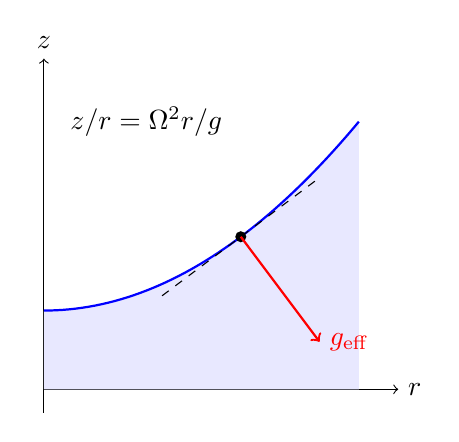
\begin{tikzpicture}[x=1cm,y=1cm]
\draw[->](0,-.3)--(0,4.2)node[above]{$z$};\draw[->](0,0)--(4.5,0)node[right]{$r$};
\fill[blue!9](0,0)--(4,0)--(4,3.4)--plot[domain=4:0,samples=50](\x,{1+.15*\x*\x})--cycle;
\draw[blue,thick,domain=0:4,samples=50]plot(\x,{1+.15*\x*\x});
\fill(2.5,1.9375)circle(2pt);\draw[->,red,thick](2.5,1.9375)--(3.5,.604)node[right]{$\bm g_{\rm eff}$};
\draw[dashed](1.5,1.1875)--(3.5,2.6875);\node at(1.3,3.4){$\dd z/\dd r=\Omega^2r/g$};\end{tikzpicture}}
图\ref{fv:n3:liquid}中液体随容器稳定转动，在转动系相对静止。局部有效重力由向下的 $g$和向外的 $\Omega^2r$合成；自由表面压强处处相同，沿面不能有压强梯度，因此表面必须垂直该合矢量。于是 $g\dd z=\Omega^2r\dd r$。以轴心液面 $(0,z_0)$ 为起点，沿表面积分：
\[
g\int_{z_0}^{z}\dd\zeta=\Omega^2\int_0^r s\,\dd s,
\qquad g[\zeta]_{z_0}^{z}=\Omega^2[s^2/2]_0^r.
\]
这给出 $g(z-z_0)=\Omega^2r^2/2$，与前面的压强法得到同一抛物面。常数 $z_0$还须由总体积确定，不能把原液面高度直接当作旋转后的轴心高度。


\section{有质量弹簧的材料微元}
\subsection{局部劲度与轴向力分布}
轻弹簧常用端点力代表整根弹簧内力；弹簧自身有质量时，各截面内力一般不同。设弹簧自然长 $L_0$、均匀质量 $m_0$、整体劲度系数 $k$。按自然坐标 $u$ 取长度 $\dd u$ 的一段，其质量为 $(m_0/L_0)\dd u$，局部劲度为 $kL_0/\dd u$，因为这些小段串联后的整体劲度必须回到 $k$。

局部轴力为 $T(u)$ 时，该微元伸长为 $\dd\ell=T(u)\dd u/(kL_0)$。所以总伸长不是某个端点力简单除以 $k$，而是
\[\Delta L=\frac1{kL_0}\int_0^{L_0}T(u)\dd u.\]
\fig{n3t-spring}{材料坐标标记同一段弹簧，伸长后位置由 $r(u)$ 给出}{\begin{tikzpicture}
\draw[axis](0,0)--(5,0)node[right]{$u$};\draw[world](0,0)--(4,0);\draw[line width=2pt,blue](1.6,0)--(2.2,0);\node[above]at(1.9,0){$\dd u$};\draw[spring](0,-1.3)--(4.8,-1.3);\draw[guide](1.6,0)--(1.8,-1.3) (2.2,0)--(2.6,-1.3);\node[below]at(2.2,-1.3){$\dd r$};\node at(3.9,.6){自然长 $L_0$};
\end{tikzpicture}}
\fig{n3deep:element}{同一材料微元两端轴力之差决定它的加速度}{\begin{tikzpicture}
\draw[spring](-2,0)--(-.6,0);\draw[spring](.6,0)--(2,0);\draw[fill=blue!8](-.6,-.25)rectangle(.6,.25);\draw[force,blue](-.6,0)--(-1.8,0)node[above]{$T(u)$};\draw[force,blue](.6,0)--(2.5,0)node[above]{$T(u+\dd u)$};\draw[dim](-.6,-.8)--(.6,-.8)node[midway,below]{$\dd r=r'(u)\dd u$};\node at(0,1){$\dd m=(m_0/L_0)\dd u$};\draw[flow](2.7,-.2)--(3.8,-.2)node[right]{$a$};
\end{tikzpicture}}
图\ref{n3deep:element}向右为正，若单位质量所受轴向体积力为 $b$，微元方程是
\[
T(u+\dd u)-T(u)+\frac{m_0}{L_0}b\dd u
=\frac{m_0}{L_0}a\dd u,
\qquad T'(u)=\frac{m_0}{L_0}(a-b).
\]
图中实际长度为 $\dd r$，自然长度为 $\dd u$，相减才是伸长；因此 $T=kL_0(r'-1)$。受力方程决定轴力怎样变化，胡克关系把轴力换成形变，两者须使用同一个材料坐标。

\subsection{自重、端点拉力与旋转的区别}
竖直悬挂弹簧时，某截面承担下方弹簧的重力，轴力随材料坐标线性改变；两端不等拉力使弹簧共同加速时，截面轴力也呈线性，但端点边界由两个拉力给定，不能只取它们的差。旋转弹簧则不同：微元向心力取决于伸长后的半径 $r(u)$，需要把受力梯度同 $r(u)$ 的局部伸长关系联立。

图\ref{n3t-spring}中的 $u$ 是材料标记，$r$ 是实际位置，两者的微元不能混用。自然坐标的质量密度为常数，但伸长后的空间线密度会改变。统一使用 $u$ 后，质量守恒自动保留，避免在求轴力时又悄悄假设伸长后的弹簧仍保持均匀空间密度。线弹性和细长模型也有适用范围，预测的伸长很大时应先检查材料是否还服从胡克定律。

相邻材料微元还使我们看清“稳定形变”的含义。弹簧整体可以平移加速，而每一材料点之间的距离在共同加速系内不再变化，这时轴力梯度承担各微元的惯性力，仍能有确定的静态形变分布。突然施力的瞬间则可能激发轴向弹性波，端点力改变并不立即使整根有质量弹簧进入上述分布。轻弹簧的瞬时模型与有质量弹簧的准稳态模型属于不同理想化；解题应分别说明考察的是瞬间、稳定旋转还是振动已可忽略的共同加速状态。
